\documentclass{article}[a4]
\usepackage[utf8]{inputenc}
\usepackage{authblk}
\usepackage{tabularx}
\usepackage{url}
\usepackage{verbatimbox}
\usepackage{graphicx}
\graphicspath{{images/}}

\title{Proposal of Automatic Extraction Framework of Superconductors related Information from Scientific literature}

\author[1]{Luca Foppiano\thanks{FOPPIANO.Luca@nims.go.jp}}
\author[1]{Thaer M. Dieb\thanks{MOUSTAFADIEB.Thaer@nims.go.jp}}
\author[1]{Akira Suzuki\thanks{SUZUKI.Akira3@nims.go.jp}}
\author[1]{Masashi Ishii\thanks{ISHII.Masashi@nims.go.jp}}
\affil[1]{Research and Services Division of Materials Data and Integrated System (MaDIS), National Institute for Materials Science (NIMS), 1-2-1 Sengen, Tsukuba, Ibaraki 305-0047, Japan}

% \date{April 2019}

\begin{document}

\maketitle

\begin{abstract}
Automatic collection of materials information from research papers using Natural Language Processing (NLP) is highly required for rapid materials development using big data, namely materials informatics (MI). Difficulty of this automatic collection is mainly caused by the variety of expressions in the papers, a system with tolerance to such variety is required to be developed. 
In this paper, we report an ongoing interdisciplinary work to construct the system for automatic collection of superconductor-related information from scientific literature using text mining techniques. 
We focus on identification of superconducting material names and their key property of critical temperature (Tc). We discuss the construction of a prototype for extraction and linking using machine learning (ML) techniques for the physical information collection.
%From evaluation using 500 sample documents, we define a baseline and a direction for future improvements.
\end{abstract}

%% The table of content is there just for organisation purposes, will be removed 
\pagebreak


\section{Introduction}
% What is the problem we are trying to solve? What are the motivation behind this project? 

Automatic information extraction from research papers using Natural Language Processing (NLP) is a highly required approach in many domains. In material research, the use of big data obtained experimentally, known as Material Informatics (MI), may give insight leading to new breakthrough in materials discovery. 
The increasing availability of scientific papers and the expertise costs to manually extract valuable data justify needs of Text and Data Mining (TDM) automatic approaches. Despite the general understanding of necessity of TDM, variation of description even in a single topic makes this task particularly complex. 
In this paper, we propose a framework for automatic data extraction and tried an actual application of this system to a scientific filed, superconductivity.  
%% How research is made and what are the point of improvements?
\textit{Superconductivity is a phenomenon of exactly zero electrical resistance and expulsion of magnetic flux fields occurring in certain materials called superconductors, under a characteristic critical temperature}~\cite{wikipedia:superconductivity}. 
Historically, high-temperature superconductors have been suddenly discovered by intuition of scientists rather than systematic consideration because of the lack of theoretical understanding \cite{klintenberg2013possible} \cite{DBLP:journals/corr/abs-1812-01995}. In this severe situation, data-driven exploration \cite{doi:10.1080/14686996.2018.1548885}, \cite{HAMIDIEH2018346} \cite{PhysRevMaterials.2.024802} \cite{doi:10.1021/cm503507h} would be a feasible approach to discover new superconducting materials. Since it requires huge data sets for precise prediction, high-throughput experiments, first-principle calculations, existing material databases should be used as data source. 

%It requires huge data sets for precise prediction, and high-throughput experiments, first-principle calculations, and existing material databases should may be useful data sources. 

Currently, several material databases are available for property search, however when looking at the superconductor sub-domain, the main one is SuperCon~\cite{SuperCon} hosted and maintained by the National Institute for Materials Science (NIMS). The SuperCon contains about 32k inorganic and about 558 organic superconductor material definitions. Although it is constantly updated with manual data collection, it cannot catch up with the massive fresh information from the increasing number of articles each year. It is our challenge to make SuperCon richer for data-driven science.

%The research in superconductor materials is articulated toward many different objectives. Discovery of new characteristic of well known materials, under new environment condition, like applied pressure or magnetic field. Combination of known superconductors with non-superconductors may lead to new materials with better characteristics, usually a higher critical temperature. 

% Add that introduction about the available databases, in particular NIMS, which has the problem that is not updated due to high costs of manual work
%Currently there are several general material databases available, however when looking  at the superconductor sub-domain the main one is SuperCon\cite{SuperCon}. Hosted and maintained by the National Institute for Materials Science (NIMS) containing about 32k inorganic and about 558 organic superconductor material definitions. Although the update continues manually, the latest information can not keep up with the increase in the enormous number of articles each year. 

% Why do we need such information? Why these information are important?
%The availability of material information with detailed and precise granularity is a must-have for superconductors scientists. This data summarises decades of research and discoveries and can be potentially exploited in many areas. Machine learning or neural models can train generative models specialised in automatically predict critical temperature \cite{DBLP:journals/corr/abs-1812-01995} on new (pure or intercalated) materials. Large scale repositories with enhanced search specialised in semantic superconductor disambiguation, document recommendation, and so on. 

In this paper we describe the ongoing attempt to design a TDM system using NLP techniques. In particular, we focus on extracting superconducting materials names and their linking with corresponding critical temperature (Tc) values.
Our system is built on an Open Source library for text mining for scholarly documents: Grobid \cite{GROBID}. We evaluate the performance of the system using precision, recall and F1-score. Such performance provides baseline for measuring our progress in solving the task.
Similar attempts of mining scientific literature in materials domain had been conducted \cite{nanocrystal_extraction} \cite{court2018auto}. 

This paper is organised as follows, Section \ref{sec:architecture} describes the details of a working prototype specialised in superconductors data extraction including the development of an annotated corpus for material names recognition. Section \ref{sec:experiments-results} presents the evaluation methods and results, section \ref{sec:conclusion} concludes the paper.

\section{System architecture}
\label{sec:architecture}
The scientific information in articles is often presented in tables and figures for easy understanding. However, in order to achieve higher order data structuring, it is necessary to link extracted entities. For example, the superconductor’s name with various expressions should be appropriately linked to corresponding property values depending on various material-measurement parameters, such as dopant density and stoichiometry or the material parameter and applied magnetic field for the measurement parameter. Obviously, these relational entities are not fully included in the tables and figures. Therefore, we insist on extracting information existing in the main body text and in captions of tables and figures. In superconductor sub-domain, since linking superconductor material with its corresponding Tc is crucial, we constructed a system for linking the material and Tc (material-Tc). Other properties, such as critical magnetic field (Hc) will be targeted in the upcoming work.

We built our implementation based on an open source library called Grobid \cite{GROBID}. Grobid is a sequence labelling and document segmentation library based on machine learning, Conditional Random Field (CRF) \cite{lafferty2001conditional}. It provides full support for extraction of data from PDF and a build-in workflow for pre-annotating training data, evaluation and training. The PDF support in Grobid was important because allowed to work with a single format instead of dealing with several XML flavours dependent on external publishers. Among various available open source tools, the choice of Grobid is well justified by the fact that it is still actively developed and it is available as ready product employed in several large scale research repositories, like for example Mendeley \cite{mendeley-extraction}. In a recent benchmark study Grobid performed best in citation extraction task \cite{DBLP:journals/corr/abs-1802-01168}. Lastly, Grobid has been successfully extended to support several domains specific problems, for example astronomical entities recognition \cite{grobid-astro}, dictionaries segmentation \cite{khemakhem2017automatic}, software mention \cite{software-mentions} and measurements extraction and normalisation \cite{grobid-quantities}. The availability of an open source measurement recognition, Grobid-quantities was fitting in our use case for Tc recognition. 

\begin{figure}[]
    \centering
    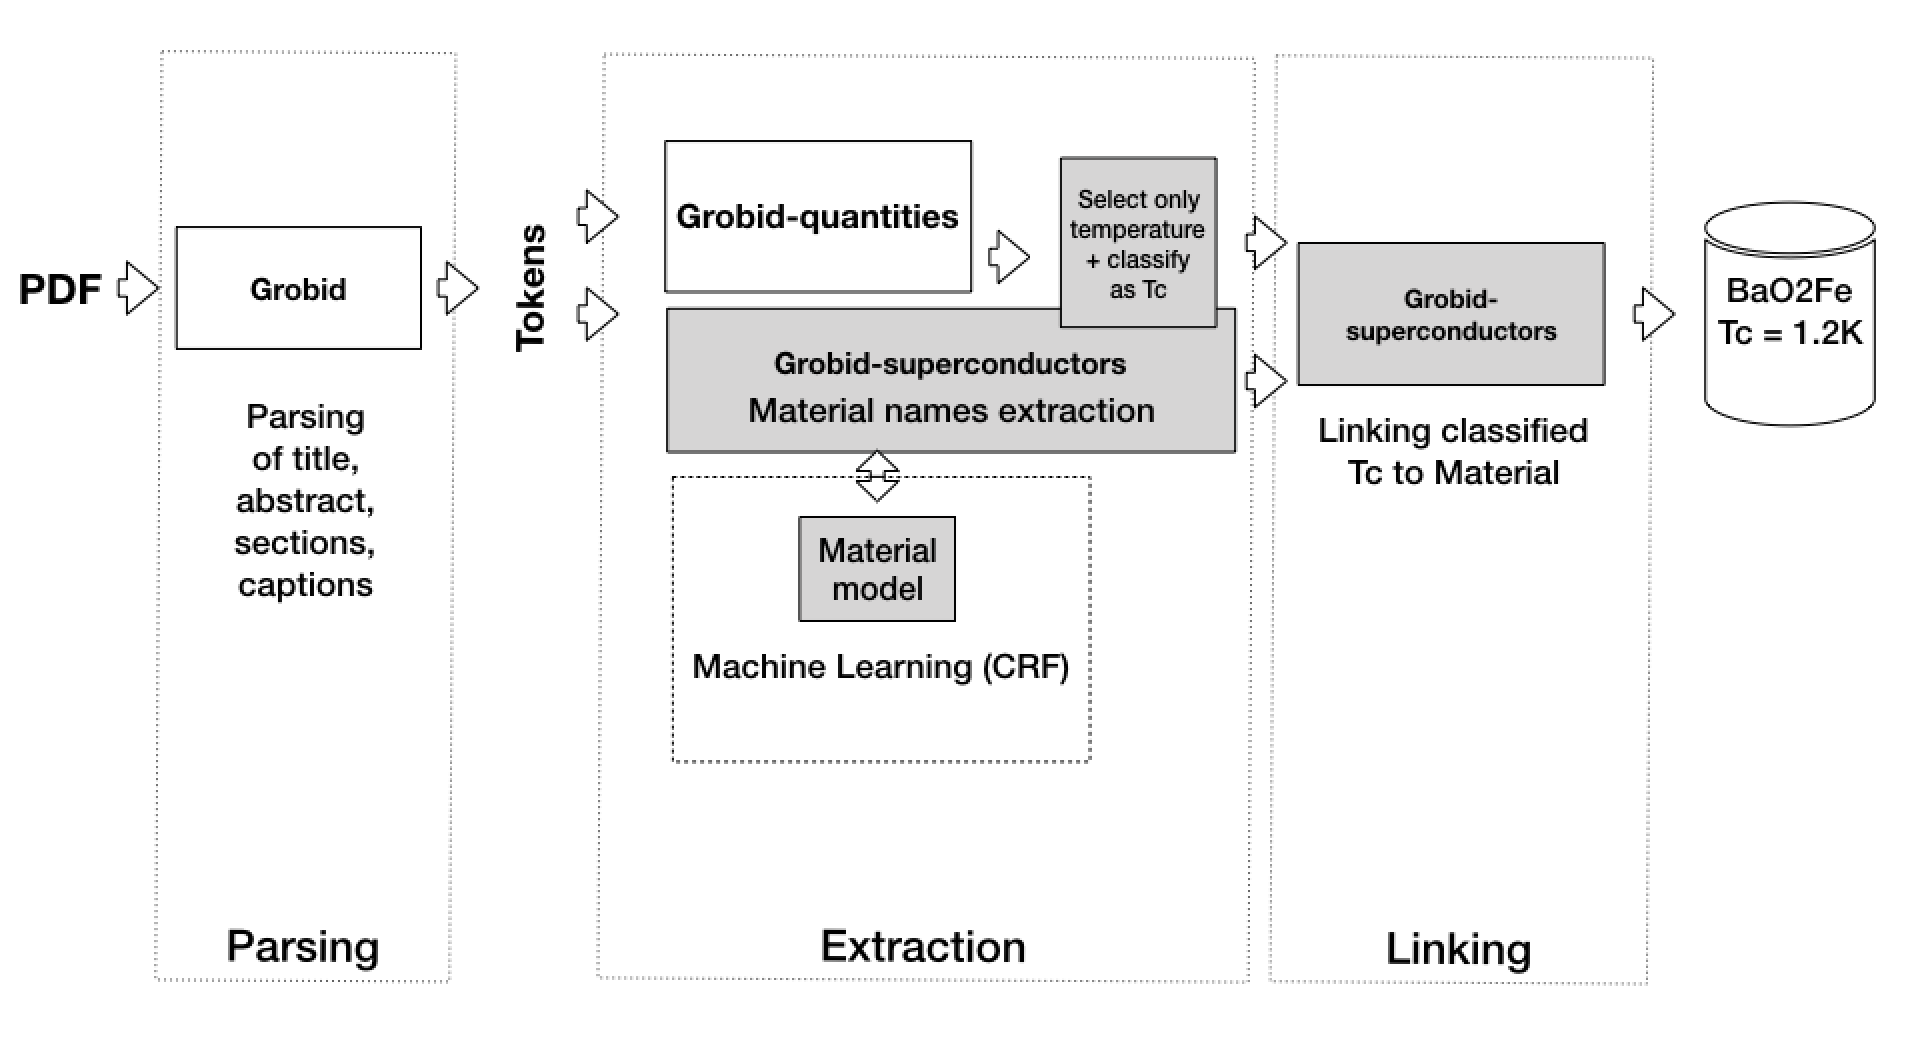
\includegraphics[width=4in]{schema}
    \caption[Schema of the system] {Schema of the system}
    \label{fig:system-schema}
\end{figure}

Our developed system illustrated in Figure \ref{fig:system-schema} consists mainly of two phases: (a) “Extraction phase” and (b) “Linking phase”. In the first phase we extract relevant entities, i.e., superconducting materials and Tc, and in the second phase, we link these extracted entities.

After parsing title, abstract, sections, and captions and following tokenisation, the (a) Extraction phase combines the entities resulting from a newly trained model for superconductor material recognition and a conventional module, Grobid-quantities for measurement extraction. The superconducting material recognition model was trained with five full documents manually annotated (42 entity in total). We also used domain-specific chemical recogniser, called ChemSpot \cite{10.1093/bioinformatics/bts183} which extracts chemical entities from text and classify them by type: SYSTEMATIC, IDENTIFIER, FORMULA, TRIVIAL, ABBREVIATION, FAMILY, MULTIPLE and UNKNOWN.

In the following (b) Linking phase, three tasks are sequentially performed: (1) since Grobid-quantities provides non-specific measurements (temperatures, lengths, pressures, etc.) including measurements unrelated to our purpose,  we selected only temperatures, then (2) we classified each of them into "Tc" and the others. Finally (3) we linked Tc with the positionally closest material term. 
The selection of Tc (2) was realised by word matching to an original dictionary, which summarises commonly used Tc-related words in superconducting literature (e.g. “Tc”, “critical temperature”). We looked for the Tc-related words in the surroundings (within five words according to empirical probability) of a numerical temperature value. 
At last, (3) the closest material term was linked to the pair of Tc and value, resulting in the required entity linking of material-Tc-value. We limited the search span at \textit{sentence level} and \textit{paragraph level} by constraining the search at the same sentence or at the same paragraph respectively (Table \ref{table:result-linking}).
This simple algorithm allowed us to prototype rapidly and implement an end to end process able to extract annotations directly from PDF and transfer them in a database. In Figures \ref{fig:example-working} and \ref{fig:example-not-working} we show two examples of correct and incorrect linking respectively, including missing extraction. 

\begin{figure}[h]
    \centering
    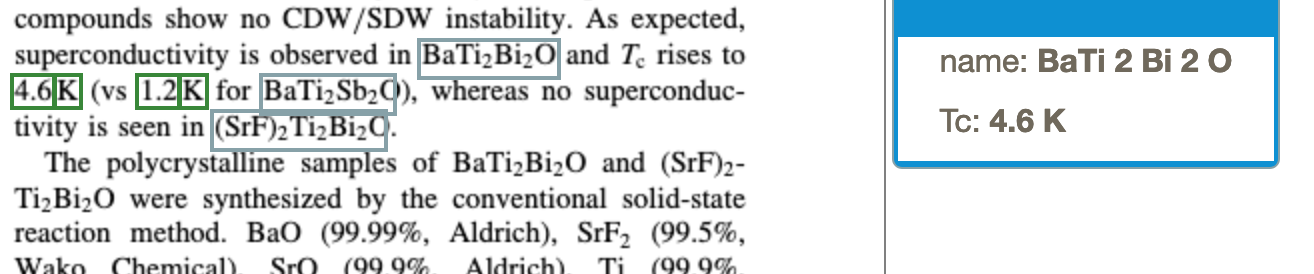
\includegraphics[width=4in]{example1} 
    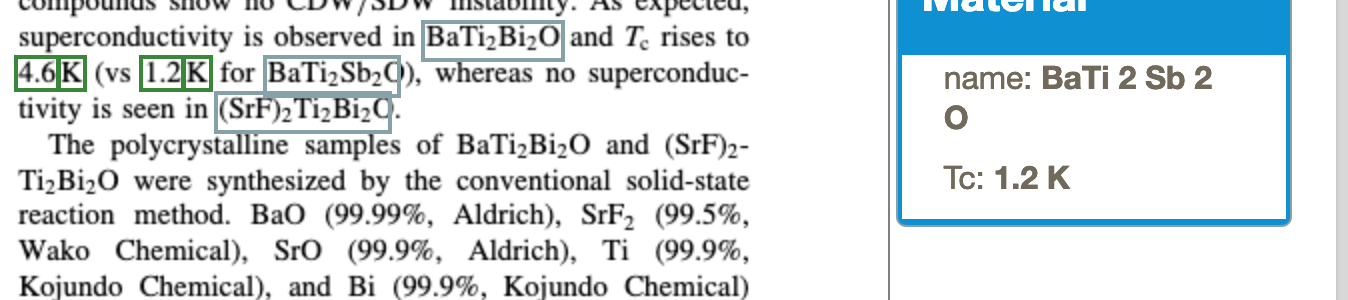
\includegraphics[width=4in]{example2}
    \caption{Example of a correct linking between material and Tc. The popup windows indicate the links of material BaTi\textsubscript{2}Bi\textsubscript{2}O with Tc of 4.6K and BaTi\textsubscript{2}Sb\textsubscript{2}O with 1.2K}.
    \label{fig:example-working}
\end{figure}

\begin{figure}[h]
    \centering
    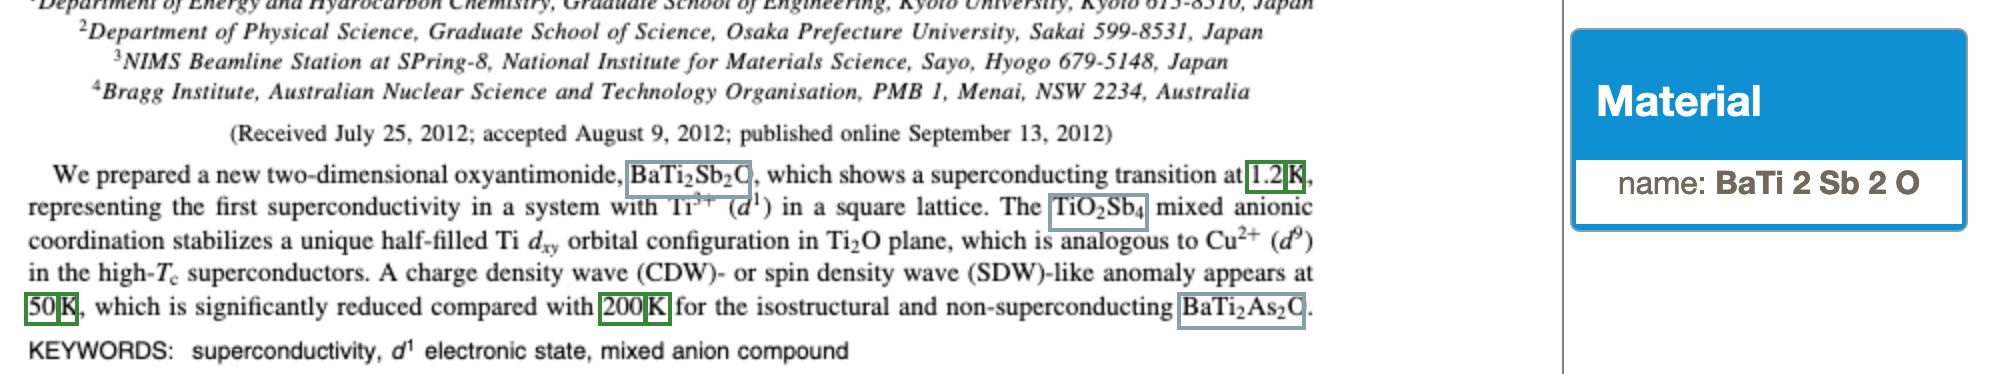
\includegraphics[width=4in]{example-bad1} 
    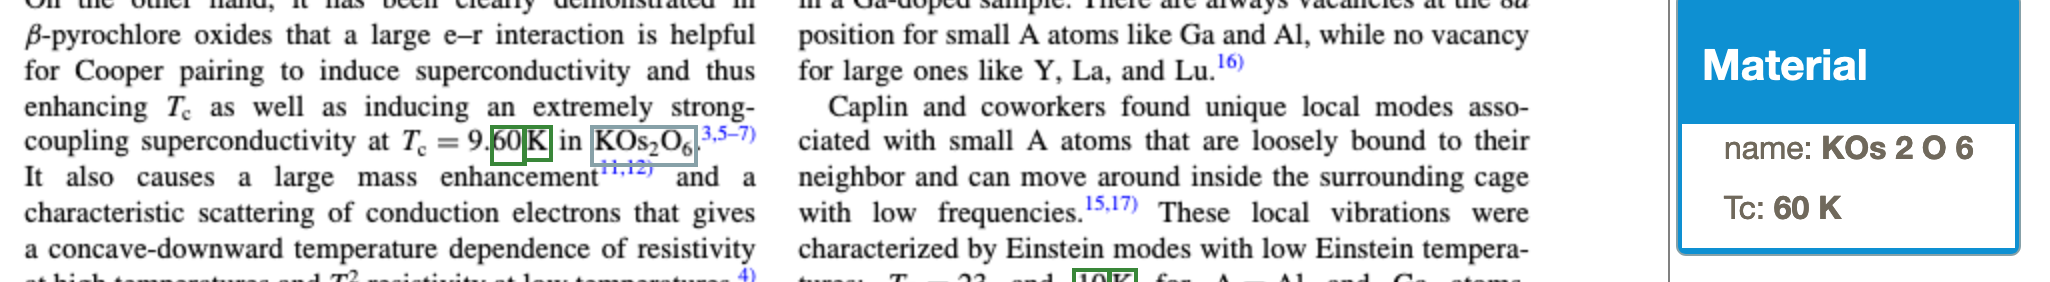
\includegraphics[width=4in]{example-bad2}
    \caption{Example of an incorrect linking between material and Tc. Although the materials BaTi\textsuperscript{2}Sb\textsuperscript{2}O and KO\textsuperscript{S2}O\textsubscript{6} are correctly identified, Tc of BaTi\textsuperscript{2}Sb\textsuperscript{2}O cannot be extracted and that of KO\textsuperscript{S2}O\textsubscript{6} is extracted incorrectly (correct Tc was 9.60 K while the extracted value was 60 K). }
    \label{fig:example-not-working}
\end{figure}

\section{Experiments and results}
\label{sec:experiments-results}
The superconductor CRF model in the (a) Extraction phase was investigated using a corpus of five papers (four for training and one for testing) having a total of 42 entities classified with a superconducting material label \textless supercon\textgreater.

\begin{figure}[h!]
    \centering
    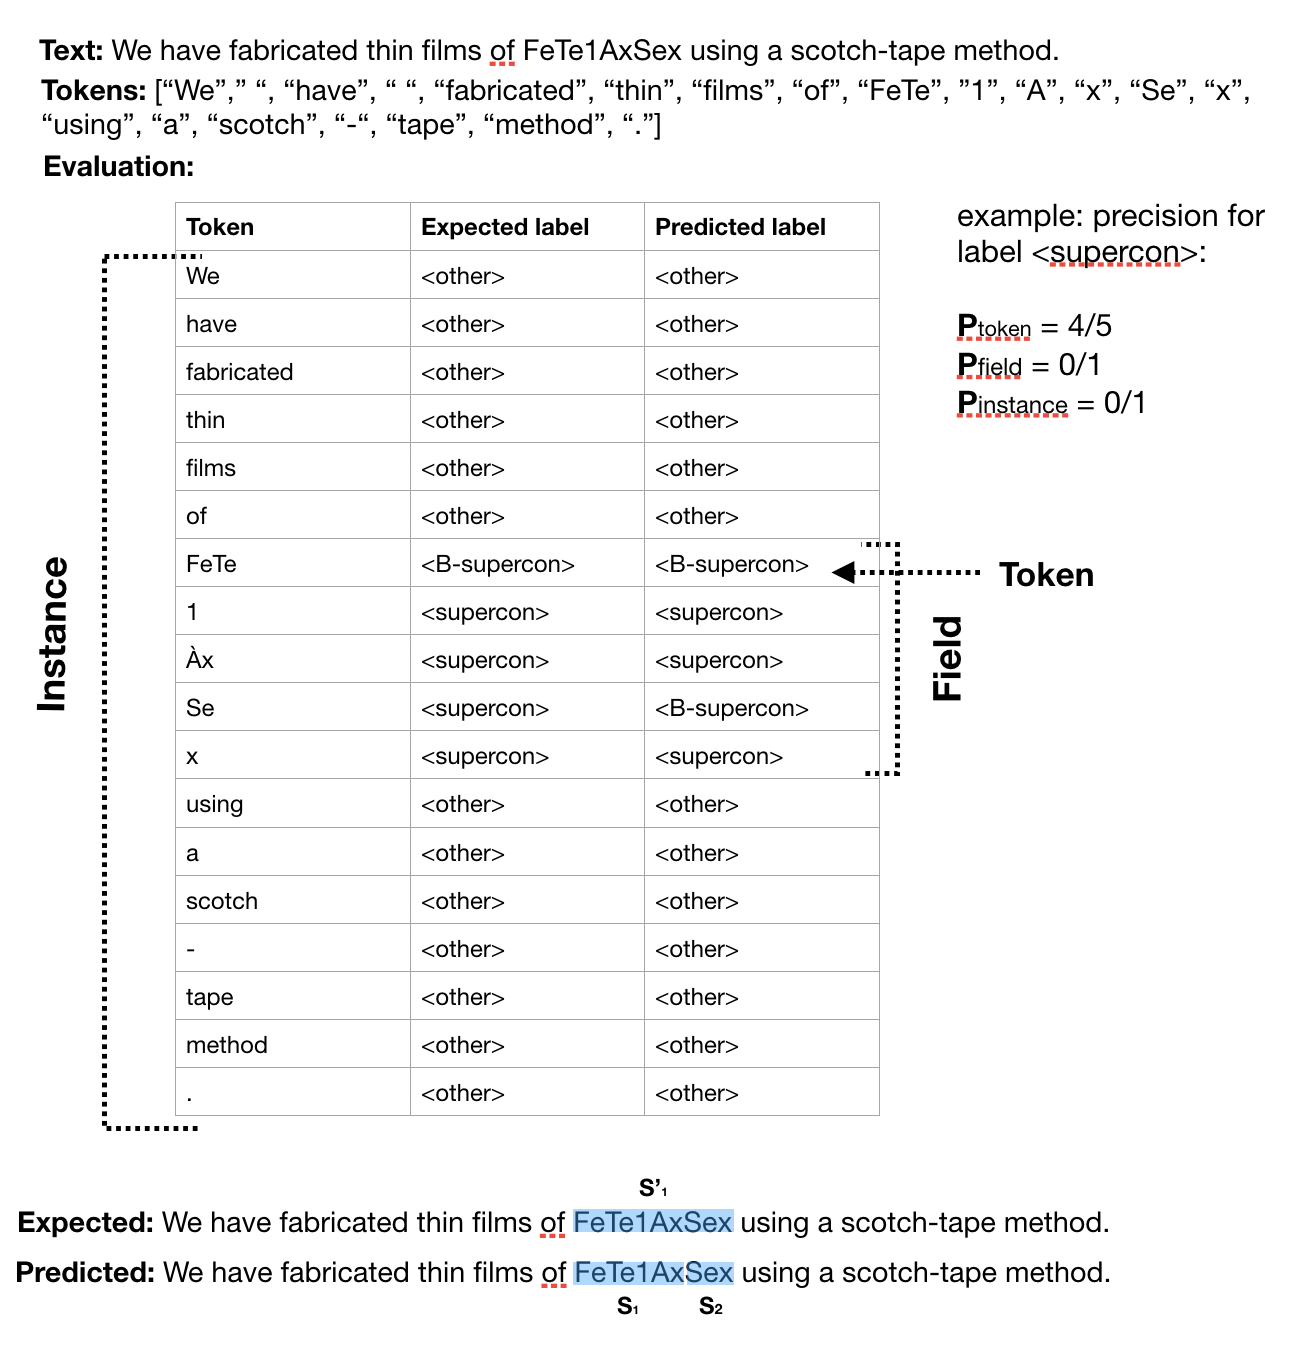
\includegraphics[width=4in]{example-output}
    \caption{Given a sentence (or paragraphs) the tokenisation transform it in an array of character sequences. These are then labelled by the ML CRF model. This figure illustrate the three different levels of granularity on which measurements are calculated.}
    \label{fig:levels-measurement}
\end{figure}

We estimated precision, recall and F1-score for the model using the evaluation framework built-in in Grobid. These measure indices are calculated at three different levels: tokens-level, field-level and instance-level. Figure \ref{fig:levels-measurement} illustrates a prediction example for explanation of the level. 
In this table, expected (second column) and predicted (third column) labels are tagged on to each token. 
The token-level evaluates the predictability for each token. Therefore, in this case, the predictability in token-level, P\textsubscript{token} is 4/5. The field-level evaluate continuity of a field with the same label. In the example, although ”FeTe\textsubscript{1}A\textsubscript{x}Se\textsubscript{x}” should be recognised as a field, the predicted label indicated separation into two fields of ”FeTe\textsubscript{1}A\textsubscript{x}” and ”Se\textsubscript{x}”. Therefore, the predictability in field-level, P\textsubscript{field} is 0/1. Finally, instance-level indicates predictability of P\textsubscript{field} in a instance, where instance is defined by a paragraph in this case. 
If ”FeTe\textsubscript{1}A\textsubscript{x}Se\textsubscript{x}” is only one field in the paragraph, the predictability in instance-level, P\textsubscript{instance} is 0/1. The predictability of P\textsubscript{token}, P\textsubscript{field}, and P\textsubscript{instance} are statistically extendable to more strict indices of precision, recall, and F1-score.

The following table illustrate Precision, recall and F1-score for our trained model.

\begin{verbnobox}[\small]
===== Token-level results =====

label                accuracy     precision    recall       f1     

<supercon>           98.61        84.42        85.28        84.85  

all fields           98.61        84.42        85.28        84.85   (micro average)
                     98.61        84.42        85.28        84.85   (macro average)

===== Field-level results =====

label                accuracy     precision    recall       f1     

<supercon>           72.94        66.67        56.25        61.02  

all fields           72.94        66.67        56.25        61.02   (micro average)
                     72.94        66.67        56.25        61.02   (macro average)

===== Instance-level results =====

Total expected instances:   22
Correct instances:          15
Instance-level recall:      68.18
\end{verbnobox}

As shown in this table, token-level, field-level, and instance-level were 85.28, 56.25, and 68.18 \%, respectively. The minimum recall at the field-level indicates insufficient training for recognition of superconducting compounds, rather than superconducting elements. The higher score at instance-level suggests that some specific superconducting compounds which are intensively appeared in a paragraph have never been trained at this stage. Moreover, the fact that the precision (66.67\%) is better than the recall (56.25\%) in the field-level indicates false positive (FP) is smaller than false negative (FN). Consequently, the true superconducting compounds are relatively difficult to recognise for our trained model (c.f., Figure \ref{fig:levels-measurement}). We have already found that missing annotation in the training papers, and so a quality improvement of training data is necessary to establish a practical extraction system.

Finally, we tested the proposed system on a larger corpus of papers. We processed 500 PDF superconductor-related papers from three publishers: American institute of Physics (AIP), American Physical Society (APS) and Institute of Physics (IOP) and manually evaluated the extracted critical temperatures and their link with the related material. 

As discussed in Figure \ref{fig:levels-measurement}, the material recognition in (a) the Extraction phase mistook in boundaries detection. The other examples of mistake are \textit{missing notation}: Predicted LaFe\textsubscript{x}O for expected LaFe\textsubscript{x}O\textsubscript{1-x}, and \textit{irregular separation}: Predicted single superconductor for expected two different materials separated by ”and” or a comma. 

Despite several imperfect extraction, we obtained unique material entities of 1644 from the 500 papers as shown in Table \ref{table:result-extraction}. For Tc extraction, although temperature could refer to unrelated experimental conditions or thermal treatment for sample preparation, 1173 entities of were extracted.

\begin{table}[h!]
    \centering
    \begin{tabular}{ | m{4em} | m{4em} | m{6em} | m{5em} | } 
    \hline
        Material entities & Unique material entities & Temperature entities & Tc entities \\
    \hline
        5400 & 1644 & 7554 & 1173 \\ 
    \hline
    \end{tabular}
    \label{table:result-extraction}
    \caption{Result of extraction of materials and Tc from a corpus of 500 papers.}    
\end{table}

In (b) the Linking phase we show results in Table \ref{table:result-linking} using \textit{sentence leve} or \textit{paragraph level} boundaries for material-Tc linking. Unfortunately, only 77 (sentence boundaries) and 109 (paragraph boundaries) correct links are obtained for the extracted Tc of 1173. From these values, in the case of \textit{sentence level} boundary, precision and recall were estimated to be 68.7\% and 6.5\%, respectively. \textit{paragraph level} boundary resulted in lower precision and higher recall, 57\% and 10.7\% respectively. Extending the search boundaries (sentence to paragraph) increased the F1-score from 11.87\% to 18.01\%. The precision drop was compensated by a recall recovery for paragraph boundaries. 
The generally low recall is partly caused by wrong parsing prior to (a) Extraction phase. The conversion from PDF to text unavoidably produces irregular tokens originated from wrong UTF-8 characters, stream ordering issues, and missing fonts.  Considering that we used empirical rules for linking as described in section \ref{sec:architecture}, the irregular tokens increase FN, resulting in the low recall. The effects of irregular token can be reduced by using volumes of training data from well-conducted corpus.

\begin{table}[h!]
    \centering
    \begin{tabular}{ | m{7em} | m{4em}| m{4em}| m{4em}| m{4em} | m{4em} | } 
    \hline
        Boundaries & Links & Correct links & precision & recall & F1-score \\
    \hline
            sentence level  & 112 & 77 & 68.7\% & 6.5\% & 11.87 \% \\
    \hline
            paragraph level & 191 & 109 & 57\% & 10.7\% & 18.01 \% \\
    \hline
    \end{tabular}
    \label{table:result-linking}
    \caption{Result of linking between materials and Tc.}    
\end{table}


\section{Conclusion}
\label{sec:conclusion}
In this paper, we proposed an automatic extraction of superconductor related information from scientific publications. The proposed system consists of two phases: a machine learning sequence labelling process for entity extraction (Extraction phase) and a simple rule-base for linking (Linking phase). 
We found feasibility of the sequence labelling and necessity of bulk corpus for performance improvement. The experiment in rule-base linking, irregular tokens introduced in a conversion process from PDF to text suggests to take a different approach for fully drawing out the potential ability of probability model and ML.
In the next step, we plan to test deep neural networks like Bi-LSTM+CRF approach and embedding in the Extraction phase. In order to overcome the technical barrier in PDF to text conversion process, we introduce more statistic approaches like sequence labelling for entity linking within the same sentence.

\pagebreak

\bibliography{references}
\bibliographystyle{plain}

\end{document}
